\documentclass{article}

\usepackage[main=english,vietnamese]{babel}
\usepackage[T1]{fontenc}
\usepackage[utf8]{inputenc}
\usepackage[sexy]{evan}
\usepackage{matchsticks}
\usepackage{wrapfig}
\usepackage{listings}

\newtheorem{hint}{Hint}

\title{Translation is fun}
\author{Nghia Doan}
\date{\today}

\begin{document}

\maketitle

In this article, we discuss some applications of pattern recognition in graph theory.

\begin{example*}[Match the phrases]
    
    Match the phrases in Vietnamese on the left of the table below,
    with their translations into English on the right of the table.

\begin{otherlanguage}{vietnamese}

    \begin{center}
        \begin{tabular}{|c|l|c|c|l|}
            \cline{1-2} \cline{4-5}
            1  & băng       &  & A & bouquet (a bunch of flowers)        \\ \cline{1-2} \cline{4-5} 
            2  & bó         &  & B & chalk                               \\ \cline{1-2} \cline{4-5} 
            3  & bó hoa     &  & C & circle                              \\ \cline{1-2} \cline{4-5} 
            4  & cánh hoa   &  & D & cluster                             \\ \cline{1-2} \cline{4-5} 
            5  & đá         &  & E & detour                              \\ \cline{1-2} \cline{4-5} 
            6  & đá lửa     &  & F & fire                                \\ \cline{1-2} \cline{4-5} 
            7  & đá phấn    &  & G & flint (a stone used to make sparks) \\ \cline{1-2} \cline{4-5} 
            8  & đường      &  & H & flower                              \\ \cline{1-2} \cline{4-5} 
            9  & đường vòng &  & I & ice                                 \\ \cline{1-2} \cline{4-5} 
            10 & hoa        &  & J & iceberg                             \\ \cline{1-2} \cline{4-5} 
            11 & lửa        &  & K & mountain                            \\ \cline{1-2} \cline{4-5} 
            12 & mở         &  & L & petal                               \\ \cline{1-2} \cline{4-5} 
            13 & mở đường   &  & M & pollen                              \\ \cline{1-2} \cline{4-5} 
            14 & mở mắt     &  & N & powder                              \\ \cline{1-2} \cline{4-5} 
            15 & núi        &  & O & road                                \\ \cline{1-2} \cline{4-5} 
            16 & núi băng   &  & P & rock                                \\ \cline{1-2} \cline{4-5} 
            17 & núi lửa    &  & Q & tear (as in teardrop)               \\ \cline{1-2} \cline{4-5} 
            18 & nước đá    &  & R & to make aware                       \\ \cline{1-2} \cline{4-5} 
            19 & nước mắt   &  & S & to open                             \\ \cline{1-2} \cline{4-5} 
            20 & phấn       &  & T & to pave the way                     \\ \cline{1-2} \cline{4-5} 
            21 & phấn hoa   &  & U & volcano                             \\ \cline{1-2} \cline{4-5} 
            22 & vòng       &  & V & wreath                              \\ \cline{1-2} \cline{4-5} 
            23 & vòng hoa   &  &   &                                     \\ \cline{1-2} \cline{4-5} 
        \end{tabular}
    \end{center}
    
\end{otherlanguage}

\end{example*}

\newpage

\begin{soln}
    We use a graph theory approach from the point of view of an English speaker to solve the problem.

    First, we look at the Vietnamese phrases. They are single- and double-word phrases.
    We connect the phrases in a graph so that each pair of phrases consists of a single-word phrases and a double-word phrase,
    the double-word phrase basically contains the single-word phrase. See the diagram below.

    \begin{figure}[h]
        \centering
        \begin{minipage}[t]{9cm}
            \centering
            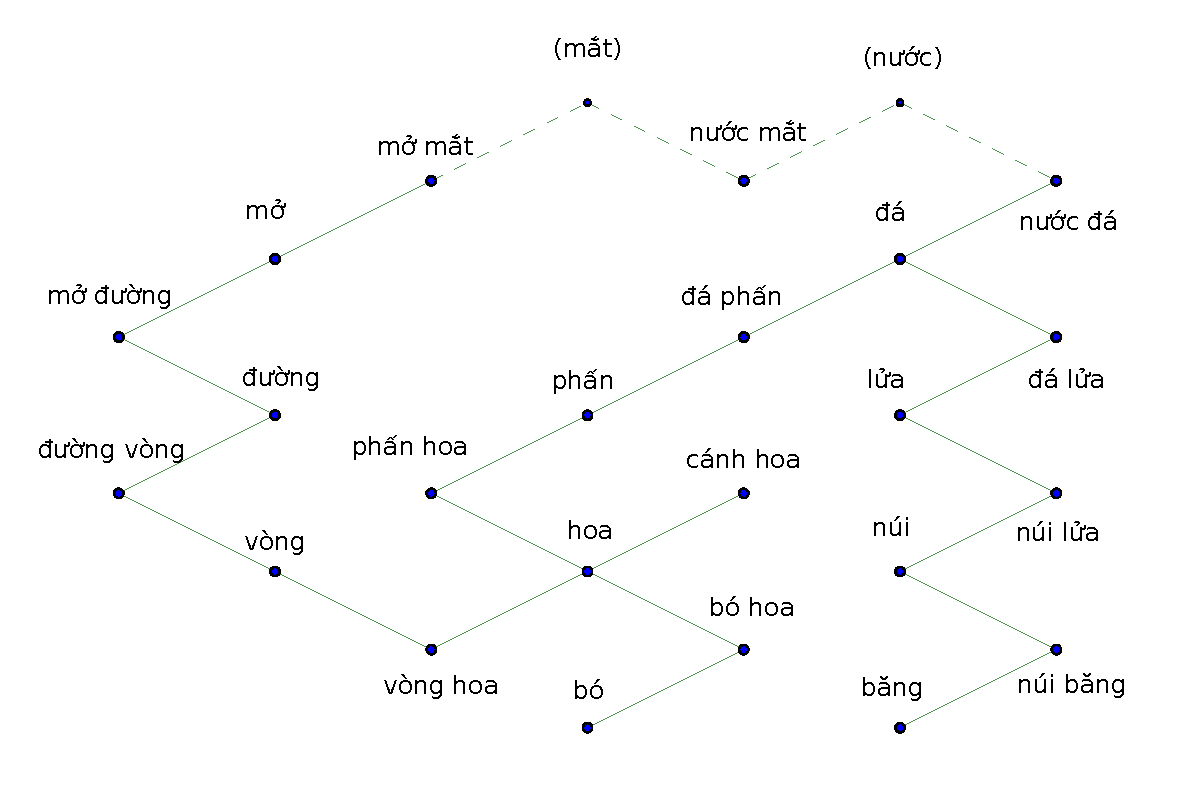
\includegraphics[width=9cm]{./svg/pdf/hc-2022-2-2-2-1.pdf}
        \caption{Graph of Vietnamese phrases}
        \end{minipage}
    \end{figure}

    The graph of Vietnamese phrases, we presume, represents connections in \textit{shared meaning} between phrases.
    Thus, we connect the English phrases in the same way,
    each phrase with another so that one has a meaning that shall be contained by the meaning of the other.
    The result is the diagram below.

    \begin{figure}[h]
        \centering
        \begin{minipage}[t]{11cm}
            \centering
            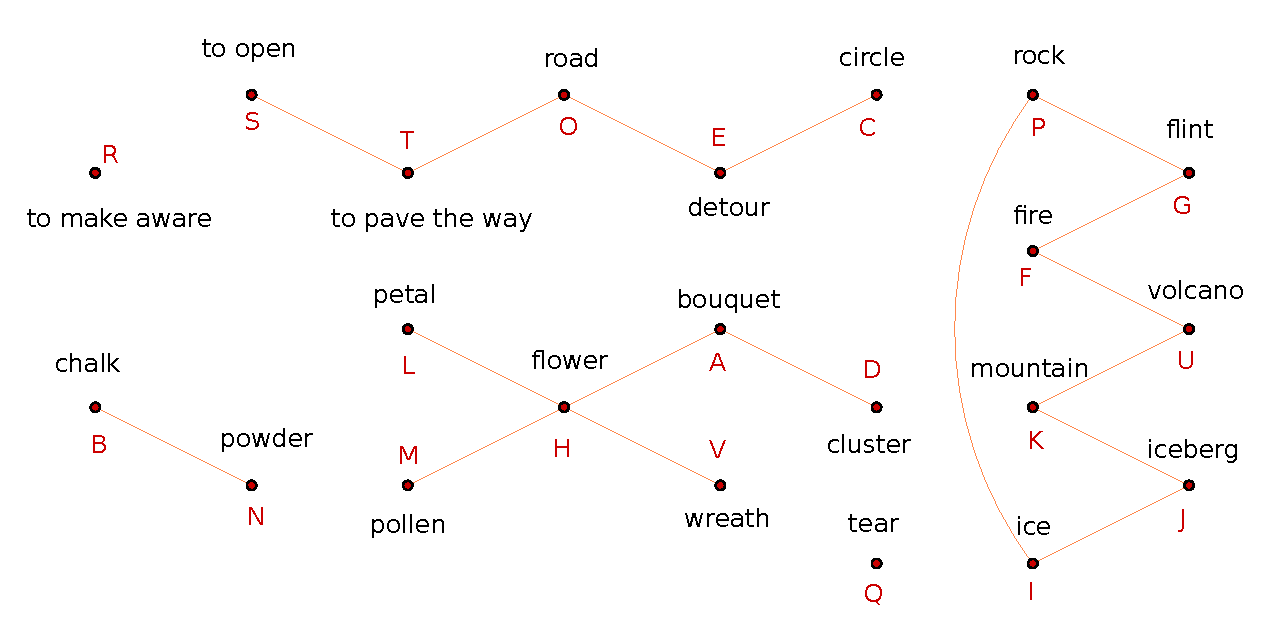
\includegraphics[width=11cm]{./svg/pdf/hc-2022-2-2-2-2.pdf}
        \caption{Graph of English phrases}
        \end{minipage}
    \end{figure}

\begin{otherlanguage}{vietnamese}

    Comparing the graph, only the $5-vertex$ subgraphs \textit{(phấn hoa, vòng hoa, cánh hoa, bó hoa, hoa)} and
    \textit{(bouquet, petal, pollen, wreath, flower),} are \textit{topologically} equivalent, thus \textit{hoa=flower}.
    Note that the relation between \textit{pollen} and \textit{powder},
    implies that \textit{powder} is \textit{phấn}. The rest of the vertices then can be paired up
    \textit{petal - cánh hoa, bouquet - bó hoa, pollen - phấn hoa, wreath - vòng hoa.}
    Therefor \textit{bó - cluster}, and \textit{chalk - đá phấn.}

    Similarly the paths \textit{(băng - núi băng - núi - núi lửa - lửa - đá lửa - đá - nước đá)} 
    \textit{(ice - iceberg - mountain - volcano - fire - flint - rock)} are very much alike,
    in addtion, the relation of \textit{đá - đá phấn} is similar to \textit{rock - chalk,}
    which make both \textit{nước đá} and \textit{băng} to have the meaning of \textit{ice}.
    Similarly the paths \textit{(vòng - đường vòng - đường - mở đường - mở)} 
    \textit{(to open - to pave the way - road - detour - circle)} are very much alike.

\newpage

    Following the reasoning, we can fill the table as shown below.

    \begin{center}
        \begin{tabular}{|c|l|l|c|l|}
            \hline
            \# & Vietnamese & Literal meaning & Answer & English       \\ \hline
            1  & băng       & ice             & I      & ice           \\ \hline
            2  & bó         & cluster         & D      & cluster       \\ \hline
            3  & bó hoa     & flower cluster  & A      & bouquet       \\ \hline
            4  & cánh hoa   & flower wing     & L      & petal         \\ \hline
            5  & đá         & rock            & P      & rock          \\ \hline
            6  & đá lửa     & fire rock       & G      & flint         \\ \hline
            7  & đá phấn    & powder rock     & B      & chalk         \\ \hline
            8  & đường      & road            & O      & road          \\ \hline
            9  & đường vòng & circle road     & E      & detour        \\ \hline
            10 & hoa        & flower          & H      & flower        \\ \hline
            11 & lửa        & fire            & F      & fire          \\ \hline
            12 & mở         & to open         & S      & to open       \\ \hline
            13 & mở đường   & to open a road  & T      & to pave a way \\ \hline
            14 & mở mắt     & to open eyes    & R      & to make aware \\ \hline
            15 & núi        & mountain        & K      & mountain      \\ \hline
            16 & núi băng   & ice mountain    & J      & iceberg       \\ \hline
            17 & núi lửa    & fire mountain   & U      & volcano       \\ \hline
            18 & nước đá    & rock water      & I      & ice           \\ \hline
            19 & nước mắt   & eye water       & Q      & tear          \\ \hline
            20 & phấn       & powder          & N      & powder        \\ \hline
            21 & phấn hoa   & flower powder   & M      & pollen        \\ \hline
            22 & vòng       & circle          & C      & circle        \\ \hline
            23 & vòng hoa   & flower circle   & V      & wreath        \\ \hline
        \end{tabular}
    \end{center}

\end{otherlanguage}

\end{soln}

\end{document}